%% V1.0
%% by Gabriel Garcia, gabrcg@gmail.com
%% This is a template for Udacity projects using IEEEtran.cls

%% Be Udacious!

\documentclass[10pt,journal,compsoc]{IEEEtran}

\usepackage[pdftex]{graphicx}    
\usepackage{cite}
\usepackage{hyperref}
% \hyphenation{op-tical net-works semi-conduc-tor}


\begin{document}

\title{Where Am I?}

\author{Lucas Wohlhart}

\markboth{Localization project, Robotics Nanodegree Program, Udacity}%
{}
\IEEEtitleabstractindextext{%

\begin{abstract}
The goal of the project at hand is the examination of the capabilities of a widely used localization technique known as Adaptive Monte Carlo Localization (AMCL).
This method is based on a particle filter algorithm which will be conceptionally compared to another localization strategy using a Kalman Filter. 
For the evaluation of the localization method, two different robots models are placed in a ROS/Gazebo/RViz simulation environment in which they have to navigate through a maze world to reach a specified goal position.
These two mobile robots both feature a differential drive, one of which is given by the Udacity project description and the creation of the second (custom) robot model will be discussed within this report.
\end{abstract}

% Note that keywords are not normally used for peerreview papers.
\begin{IEEEkeywords}
Robot, IEEEtran, Udacity, \LaTeX, Localization.
\end{IEEEkeywords}}


\maketitle
\IEEEdisplaynontitleabstractindextext
\IEEEpeerreviewmaketitle
\section{Introduction}
\label{sec:introduction}

\IEEEPARstart{T}{he} capability of accurately determining the pose of a mobile robot is a crucial necessity for being able to autonomously navigate any given environment.
The problem of localization poses three challenges to tackle, which are known as: local localization, global localization and the kidnapped robot problem.
The goal of local localization is to keep track of the pose changes due to robot movement given a known initial pose. In global localization the robots pose starts out as being unknown and the objective is to determine the pose by comparing observations to a ground truth map. The kidnapped robot problem is similar to global localization since the goal is also to find the robots pose without knowing it's initial location, but with the challenging additional constraint that the robot might be randomly placed at an entirely different spot in the world at any time. 
This project tackles the problem of global localization which, if implemented and tuned correctly, enables the robots to autonomously navigate the maze world depicted in Figure~\ref{fig:maze} to reach a specified goal pose. 


%example for inserting image
\begin{figure}[thpb]
      \centering
      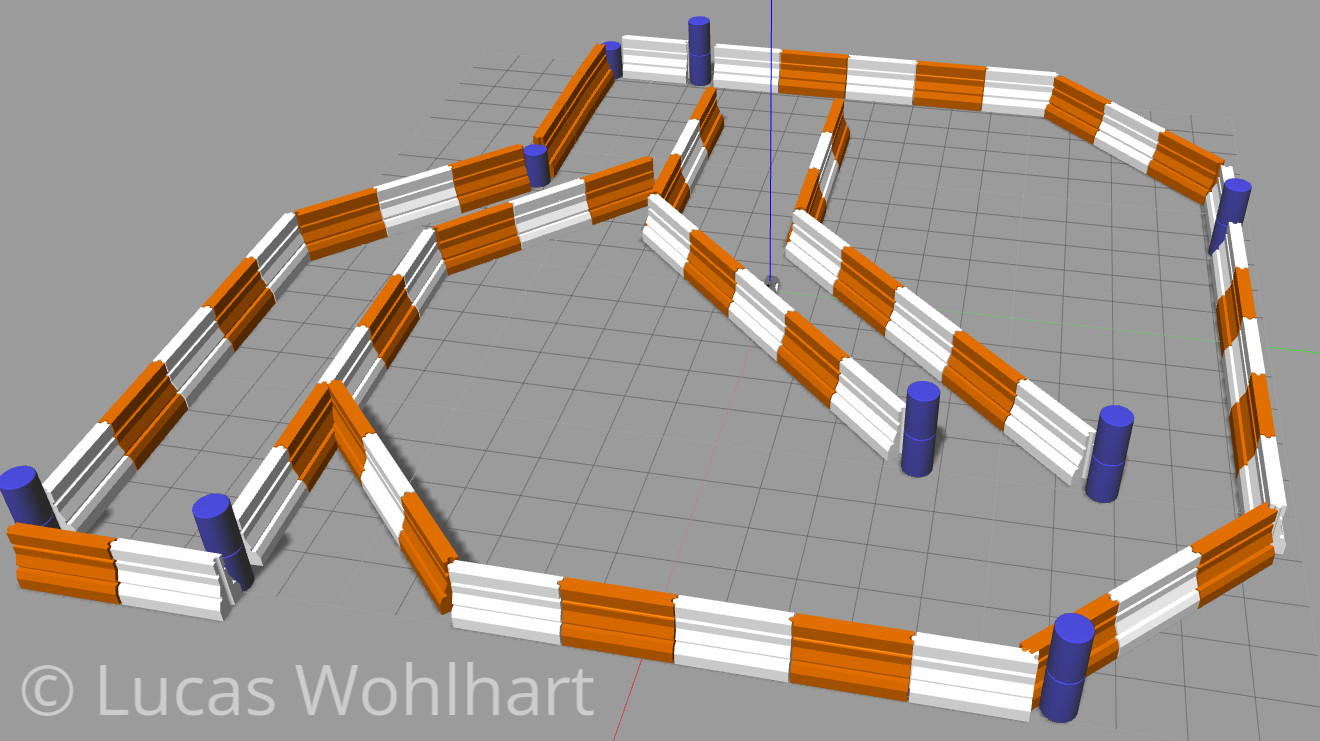
\includegraphics[width=\linewidth]{img/maze_world}
      \caption{Maze environment}
      \label{fig:maze}
\end{figure}



\section{Background}
Solving a localization problem boils down to modelling the robots pose changes resulting from the motions executed by the actuators and interpreting the available sensor readings to gather evidence from the environment which can be compared to a known ground truth map.
Both these processes are subject to noise since motions can't be performed with absolute accuracy and sensors don't capture the exact truth about the surrounding world.
The objective of a localization algorithm is therefore to filter out the motion and measurement noise and yield a robust estimation of the robots pose. 

The (Extended) Kalman Filter is a well established method for local localization and will discussed in comparison to the Adaptive Monte Carlo localization particle filter which is able to solve global localization problems.

Since in this project setup the initial pose of the robot is not known, the Adaptive Monte Carlo Localization (AMCL) method was chosen and implemented. Additionally this approach provides a simple way of modelling the nonlinear motions of the robot and is capable of solving the kidnapped robot problem as will be discussed in the following sections.

\subsection{Kalman Filters}
The Kalman Filter is a widely used state estimation algorithm which starts out with an initial state (e.g. a state vector holding the estimated x and y position and the angular orientation of a robot) as well as a covariance matrix expressing the certainty of the estimate and iteratively applies measurement updates and state predictions for each motion step of the robot.

The state prediction step takes the current motion commands of the robot, maps them to the state domain using the predefined state transition matrix and combines the result with the prior state and covariance plus additional gaussian noise to account for noisy motions. This yields the posterior belief about the robots state after a motion step.

The measurement update step uses the measurement function to map the previously calculated posterior state of the prediction step to the measurement domain. This means calculating the expected values of all available sensors, assuming the robot were in this exact state. Computing the difference between this assumption and the actual sensor readings yields the measurement residual.
The so called Kalman Gain is then computed by projecting the covariance to the measurement domain, adding potential measurement noise to all components and reprojecting this result to the state domain. This is a measure indicating the ratio of preserving the previous state estimate and taking in the new measurement evidence. It ranges from a 0-vector which keeps the previous state estimate entirely, to the pseudo inverse of the measurement function which overrides the estimate with the incoming measurement data.

Therefore the Kalman Gain is subsequently used to update the state and covariance estimate.

One drawback of the standard Kalman Filter is that it can't deal with non linear state transitions or measurement functions. Applying a non linear transformation on a Gaussian distribution yields a probability distribution which is non Gaussian and since robots usually perform non linear motions such as driving along a circle or a curve the standard Kalman Filter is not usable for most robotics applications.
To overcome this problem the Extended Kalman Filter (EKF) was introduced which linearizes the non-linear transformations by approximating them with a first order Taylor series expansion. This linearization is only valid for a small region but if the update cycles are short enough the EKF has shown to be able to produce a good and stable state/pose estimation.


\subsection{Particle Filters}
\label{sec:amcl}
A particle filter algorithm for robot localization starts by instantiating a number of uniformly distributed particles each representing one guess about the position and orientation of the robot. For every particle a weight can be calculated which corresponds to the likelihood of observing the current readings from the available range-finder sensors (e.g.  lidar, RGB-D cameras or others). If a particle matches the observation compared to the ground thruth deduced from the known map better, it gets a bigger weight than others which are less likely. Every motion step of the robot is also applied to each particle with some added noise. After a specific resample interval (usually also every motion step) the particles are then randomly resampled based on their weights and new particles might be spawned in proximity to the previously higher weighted particles. 

By iteratively applying the algorithm:
\begin{itemize}      
      \item motion update: apply robots motion with noise to each particle
      \item sensor update: assign weights to particles based likelihood of matching sensor readings
      \item resample: randomly sample current particle set and insert new particles based on weighted probabilities
\end{itemize}
the particles converge to the true pose of the robot because those which best fit the incoming evidence from the sensors have the highest chance of surviving the resample step.

If correctly configured, the Adaptive Monte Carlo Localization particle filter is even capable of solving the kidnapped robot problem by sparsely inserting particles in randomly chosen remote areas of the particle cloud which allows the algorithm to recover when losing track of the actual pose due to the kidnapping.


\subsection{Comparison / Contrast}

As outlined previously, a major advantage of the Adaptive Monte Carlo Localization method is that it isn't restricted to the assumption of a linear gaussian state space as is the case for a Kalman Filter approach. Any motion or measurement noise model can be used to compute the posterior particle estimates. Furthermore the AMCL is able to solve global localization and even the kidnapped robot problem since it doesn't require an initial state to converge. It is capable of recovering from initial or intermediate erroneous state estimates which makes filter much more robust. 

While the EKF is in general superior in terms of memory and computational efficiency as well as achievable localization accuracy the AMCL allows the user to fully take control of said parameters. By tuning the number of particles used for the filter one can adjust the tradeoff between localization accuracy and resource efficiency to fit the needs of the application.

Table~\ref{tab:mcl_ekf_comparison}, taken from the Udacity lecture "Power of MCL", summarizes the advantages and disadvantages of the discussed localization techniques.


%example for building table
\begin{table}[h]
      \caption{MCL vs EKF comparison}
      \label{tab:mcl_ekf_comparison}
      \begin{center}
            \begin{tabular}{|l||c|c|}
                  \hline
                  & MCL & EKF\\ \hline \hline
                  Measurements & Raw Measurements & Landmarks \\ \hline
                  Measurement Noise &  Any &  Gaussian \\ \hline
                  Posterior &  Particles & Gaussian \\ \hline
                  Memory Efficiency & +  & + +  \\ \hline
                  Time Efficiency&  +  & + +  \\ \hline
                  Ease of Implementation & + +  & +  \\ \hline
                  Resolution & +  & + + \\ \hline
                  Robustness & + +  & - \\ \hline
                  Memory/Resolution Control & +  & - \\ \hline
                  Global Localization & +  & - \\ \hline
                  State Space &  Multimodal Disc. & Unimodal Cont. \\ \hline
            \end{tabular}
      \end{center}
\end{table}

\section{Simulations}


% package dependencies: from clean install ( either navigation stack or separate packages: move_base, amcl, map_server ... find more)


To test the capabilities of the Adaptive Monte Carlo Localization method two robots were simulated in a ROS environment using Gazebo and RViz.

\subsection{Achievements}
After tweaking all necessary parameters for the involved software packages, both robot models were able to accurately localize themselves in the environment and successfully navigate through the provided maze.

% Robot Models
\subsection{Benchmark Model}
\subsubsection{Model design}

The baseline robot model called udacity\_bot was designed using the URDF (Unified Robot Description Format) methodology, which is a XML based description standard allowing the creator to define the topology of a robot. 
Using the SDF (Simulation Description Format), an extension to URDF introduced for Gazebo simulations, one can declare virtual sensors and actuators for the robot which are then available to use in ROS.
By creating basic geometric objects, including 3D mesh models and linking the individual parts with joint description one can easily create a simple robot which can be rendered and simulated.


The udacity\_bot is a differential drive robot consisting of a simple box shaped rigid body with support caster spheres for balance, which has a front facing camera and a laser range sensor attached. The wheels are modeled as cylinders connected with continuous joints to the rigid body.
The dimension of the individual parts is shown in detail in Table~\ref{tab:udacity_bot_model} and the resulting robot model in Gazebo simulation is depicted in Figure~\ref{fig:udacity_bot}.

\begin{table}[h]
      \caption{udacity\_bot model}
      \label{tab:udacity_bot_model}
      \begin{center}
            \begin{tabular}{|l||c|c|} 
                  \hline
                  Part & Geometry & Dimension\\ \hline \hline
                  Chassis & Cube & 0.4 x 0.2 x 0.1 \\ 
                  & Origin & x: 0.0 y: 0.0 z: 0.0 \\ \hline 
                  Back/Front caster & Sphere & radius: 0.0499 \\ 
                  & Origin & x: $\pm$ 0.15 y: 0.0 z: -0.05 \\ \hline 
                  Left/Right Wheel & Cylinder & radius: 0.1, height: 0.05 \\ 
                  & Origin & x: 0.0 y: $\pm$ 0.15 z: 0.0 \\ \hline \hline  
                  Camera Sensor & Cube &  0.05 x 0.05 x 0.05\\ 
                  & Origin & x: 0.2 y: 0.0 z: 0.0 \\ \hline 
                  Laser Range Sensor & Mesh &  0.1 x 0.1 x 0.1\\ 
                  (Hokuyo)  & Origin & x: 0.15 y: 0.0 z: 0.1 \\ \hline         
            \end{tabular}
      \end{center}
\end{table}
 

\begin{figure}[thpb]
      \centering
      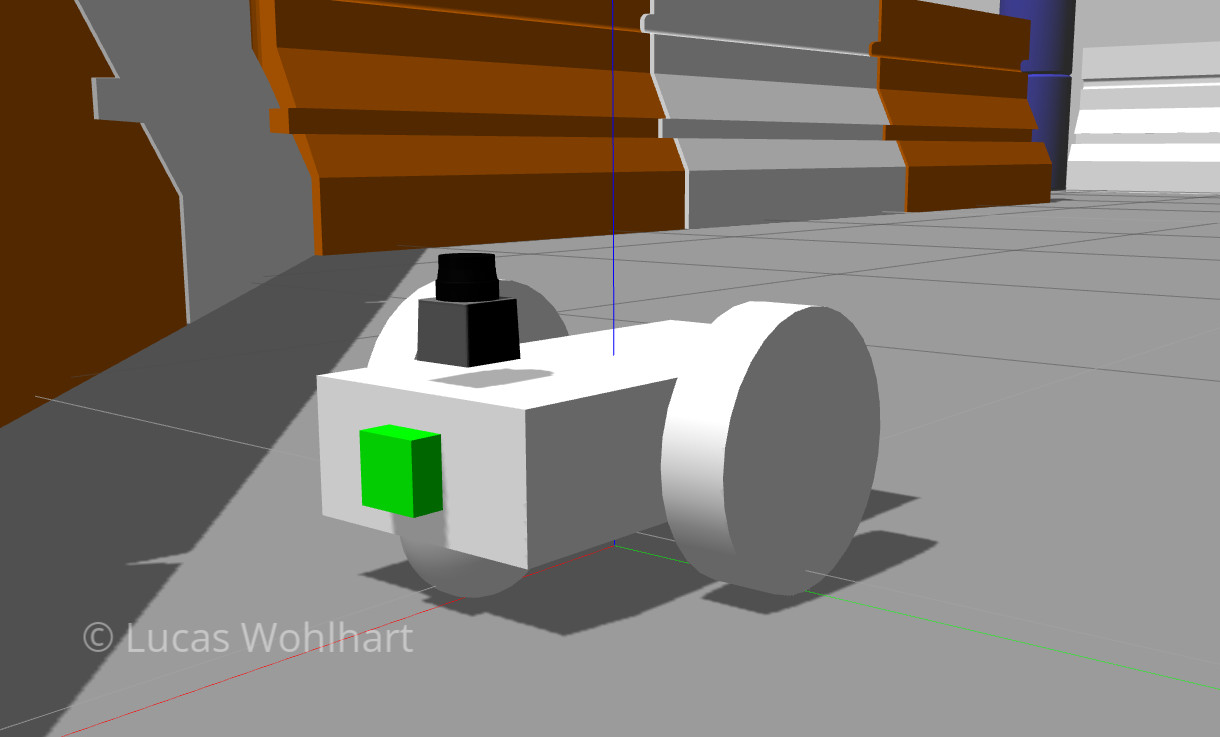
\includegraphics[width=\linewidth]{img/udacity_bot}
      \caption{Udacity Bot}
      \label{fig:udacity_bot}
\end{figure}

\subsubsection{Packages Used}
\label{sec:packages_udacity_bot}

The ROS package created for the simulation utilizes several components from the NavigationStack meta package as well as default ROS nodes. 
All necessary external packages, which are not present in the default ROS-Kinetic installation including Gazebo and RViz tooling, are declared as dependencies in the package.xml. 

Required packages:
\begin{itemize}
 \item rviz
 \item gazebo\_ros
 \item joint\_state\_publisher
 \item robot\_state\_publisher
 \item map\_server \cite{ROSNavMapServer} 
 \item amcl \cite{ROSNavAMCL}
 \item move\_base \cite{ROSNavMoveBase}
\end{itemize}

Launching the udacity\_world.launch combines all required nodes to fire up the simulation environment.
The gazebo\_ros empty\_world.launch starts a plain Gazebo physics simulation world and loads the world model declared in jackal\_race.world.
With the help of \texttt{gazebo\_ros} spawn\_model, \texttt{joint\_state\_publisher} and \texttt{robot\_state\_publisher} one can instantiate the URDF+SDF robot model defined in the robot\_description.launch file.

The \texttt{map\_server} package is used to load and publish the maze map defined in jackal\_race.yaml and jackal\_race.pgm.

Once the environment is set up, the \texttt{AMCL} node implementing the localization using a particle filter as described in section~\ref{sec:amcl} starts, subscribing to the laser scan published from the hokuyo sensor and the map.
The \texttt{move\_base} package provides the move\_base node which takes care of planning and executing the motions to navigate to a specified goal position.
A custom C++ node is included in the package which simply uses the move\_base action server to send this goal location and wait for the robot to arrive there.



\subsubsection{Parameters}

Tuning the parameters of the AMCL localization node as well as the path and motion planner node of the move\_base package to the requirements of the application is the crucial aspect to solve the localization and navigation task.
Initially following the guidelines of ROSNavigationGuide\cite{ROSNavigationGuide} and iteratively adapting the parameterization yielded the following configuration.


\begin{table}[h]
      \caption{Costmap parameterization}
      \label{tab:costmap_parameterization}
      \begin{center}
            \begin{tabular}{|l|c|}  
\multicolumn{2}{c}{Costmap common} \\ \hline 
obstacle\_range & 2.5  \\ \hline
raytrace\_range & 3.0  \\ \hline
transform\_tolerance& 0.2 \\ \hline
robot\_radius& 0.25 \\ \hline
inflation\_radius & 0.5 \\ \hline 

\multicolumn{2}{c}{Global costmap} \\ \hline 
   update\_frequency &  10.0 \\ \hline
   publish\_frequency &  5.0 \\ \hline
   width &  10.0 \\ \hline
   height &  10.0 \\ \hline
   resolution &  0.1 \\ \hline
   static\_map &  true \\ \hline
   rolling\_window &  false \\ \hline

\multicolumn{2}{c}{Local costmap} \\ \hline 
   update\_frequency &  10.0 \\ \hline
   publish\_frequency &  5.0 \\ \hline
   width &  3.0 \\ \hline
   height &  3.0 \\ \hline
   resolution &  0.1 \\ \hline
   static\_map &  false \\ \hline
   rolling\_window &  true \\ \hline
            \end{tabular}
      \end{center}
\end{table}

The parameters \texttt{obstacle\_range} and \texttt{raytrace\_range} define the distance of the laser range sensor readings to consider while updating the costmap with incoming evidence.

Since the measurement process and the update of the transformation tree is not time syncronised one has to allow for a small time delay by adjusting the \texttt{transform\_tolerance}. Though, this tolerance shouldn't be excessive because updating the map based on an outdated pose estimate deteriorates the result.

The \texttt{inflation\_radius} defines the extent to which the cost of a detected obstacle is affecting the unoccupied terrain around it.
Together with the \texttt{robot\_radius} it is used to define how strongly the navigation algorithm avoids coming close to obstacles.

Both maps are regulary updated and published with their respective frequencies.
The global costmap is a static (10x10) map covering the world while the local costmap is not static but uses the rolling window approach to model a small section of the local surroundings of the robot.
This way the local map can be relatively small (3x3) making it computationally less expensive to derive a local navigation policy. 
The resolution of both maps can be adjusted to fit the necessary granularity for collision free navigation while keeping memory and processing requirements minimal.


\begin{table}[h]
      \caption{NavFN local trajectory planner parameterization}
      \label{tab:planner_parameterization}
      \begin{center}
            \begin{tabular}{|l|c|}
      \multicolumn{2}{c}{Robot Configuration} \\ \hline
      acc\_lim\_x & 2.0 \\ \hline
      acc\_lim\_theta & 2.0 \\ \hline
      max\_vel\_x & 0.4 \\ \hline
      min\_vel\_x & 0.1 \\ \hline
      max\_vel\_theta & 1.0 \\ \hline
      min\_vel\_theta & -1.0  \\ \hline
      min\_in\_place\_vel\_theta & 0.4 \\ \hline
      escape\_vel & -0.1 \\ \hline
      holonomic\_robot & false \\ \hline

      \multicolumn{2}{c}{Forward Simulation} \\ \hline
      sim\_time & 1.5 \\ \hline
      sim\_granularity & 0.025 \\ \hline
      angular\_sim\_granularity & 0.025\\ \hline
      vx\_samples & 10 \\ \hline
      vtheta\_samples & 20 \\ \hline
      controller\_frequency & 10.0 \\ \hline

      \multicolumn{2}{c}{Trajectory Scoring} \\ \hline
      meter\_scoring & true \\ \hline
      pdist\_scale & 1.0 \\ \hline
      gdist\_scale & 0.8 \\ \hline
      occdist\_scale & 0.01 \\ \hline
      dwa & true \\ \hline
            \end{tabular}
      \end{center}
\end{table}                  

The trajectory planner uses the Dynamic Window Approach (Fox et al.\cite{Fox-1997-16403}) to derive a local navigation policy at each control cycle (\texttt{controller\_frequency}) for the command velocities of the actuators, resulting in a piecewise approximation of the path with circular arcs.
This is done by sampling directly from the subspace of rotational and translational velocities that are reachable within the next timeframe, given the current state and capabilities of the robot defined by acceleration and velocity limits.

The number of translational and rotational velocity pairs to consider can be configured with \texttt{vx\_samples} and \texttt{vtheta\_samples}. Each velocity proposal is forward simulated for a short time interval defined by \texttt{sim\_time} with a step size of \texttt{sim\_granularity} and \texttt{angular\_sim\_granularity}.
Then it is rated with regards to the objective cost function balancing the tradeoff between sticking to the proposed path (\texttt{pdist}), reaching the next local goal (\texttt{gdist}) and staying away from obstacles (\texttt{occdist}).


The particle filter implemented in the AMCL package is configured to yield satisfactory localization performance while keeping the computational load manageable.

\begin{table}[h]
      \caption{AMCL parameterization}
      \label{tab:amcl_parameterization}
      \begin{center}
            \begin{tabular}{|l|c|}  \hline
min\_particles & 50 \\ \hline
max\_particles & 200 \\ \hline
update\_min\_d & 0.1 \\ \hline
update\_min\_a & 0.26 \\ \hline
resample\_interval & 1 \\ \hline
recovery\_alpha\_slow & 0.0 \\ \hline
recovery\_alpha\_fast & 0.0 \\ \hline

initial\_pose\_x & 0.0  \\ \hline
initial\_pose\_y & 0.0  \\ \hline
initial\_cov\_xx & 20.0  \\ \hline
initial\_cov\_yy & 20.0  \\ \hline

laser\_max\_beams & 60 \\ \hline
% odom\_model\_type & diff \\ \hline
odom\_alpha1 & 0.02 \\ \hline
odom\_alpha2 & 0.02 \\ \hline
odom\_alpha3 & 0.02 \\ \hline
odom\_alpha4 & 0.02 \\ \hline
\end{tabular}
\end{center}
\end{table}                  



The main aspect to control is the amount of particles used for the filtering process. To solve the global localization problem at hand it suffices to operate with 50 to 200 particles. The \texttt{resample\_interval} of 1 ensures a resampling of the particle set after every motion step while \texttt{update\_min\_d} and \texttt{update\_min\_a} declare the minimum translational and angular change between steps to update.

Setting the \texttt{initial\_pose\_(x|y)} to (0.0, 0.0) with an \texttt{initial\_cov\_(xx|yy)} of (20.0, 20.0) expresses very high uncertainty about the initial state since this a global localization problem. The resulting initial distribution of particles is shown in Figure~\ref{fig:particles_initial_high_cov}.

The parameters \texttt{odom\_alpha\_(1,2,3,4)} specify the amount of noise added to the particles after a motion step to account for inaccurately executed motions. 

\begin{figure}[thpb]
      \centering
      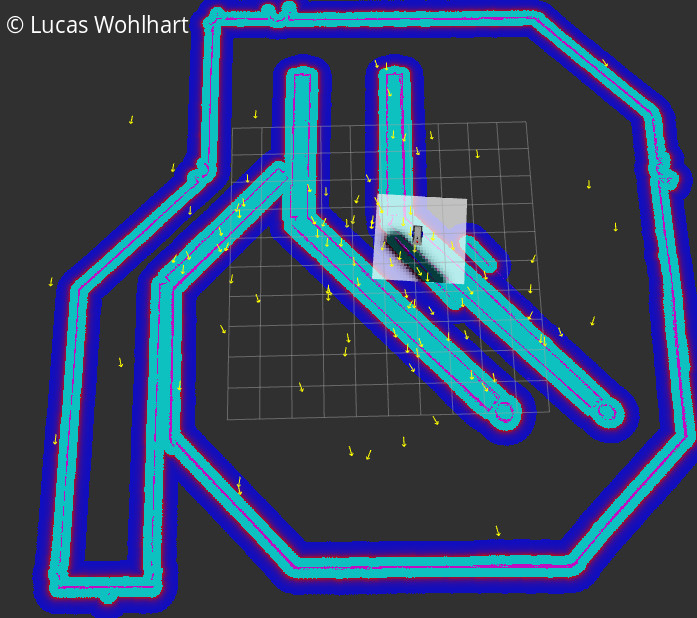
\includegraphics[width=\linewidth]{img/particles_initial_high_cov}
      \caption{Initial particle distribution}
      \label{fig:particles_initial_high_cov}
\end{figure}

One could also cope with the possibility of having to solve the kidnapped robot problem by adjust the following parameters:

\begin{table}[h]
      \caption{AMCL parameterization for kidnapped robots}
      \label{tab:amcl_parameterization}
      \begin{center}
            \begin{tabular}{|l|c|}  \hline
      kld\_err & 0.005 \\ \hline
      kld\_z & 0.95\\ \hline
      recovery\_alpha\_slow & 0.01  \\ \hline
      recovery\_alpha\_fast & 0.5  \\ \hline
      \end{tabular}
\end{center}
\end{table}        
The parameters \texttt{recover\_alpha\_(slow|fast)} control the thresholds of average particle weights needed to randomly spawn new particles in unrelated locations to recover from erroneous pose estimates.

\subsection{Personal Model}
% ditto
The custom robot model is inspired by the MSE-6-series repair droid\cite{MSE-6-series-droid} used by the Galactic Empire. 
\subsubsection{Model design}
The chassis of the MSE-6 repair droid (shown in Figure~\ref{fig:blender_design_mse6}) consists of a COLLADA mesh, modelled using the open source 3D modelling softwar blender\cite{Blender}. The format is an XML based description for digital assets exchange, which can be included in a URDF file.

\begin{figure}[thpb]
      \centering
      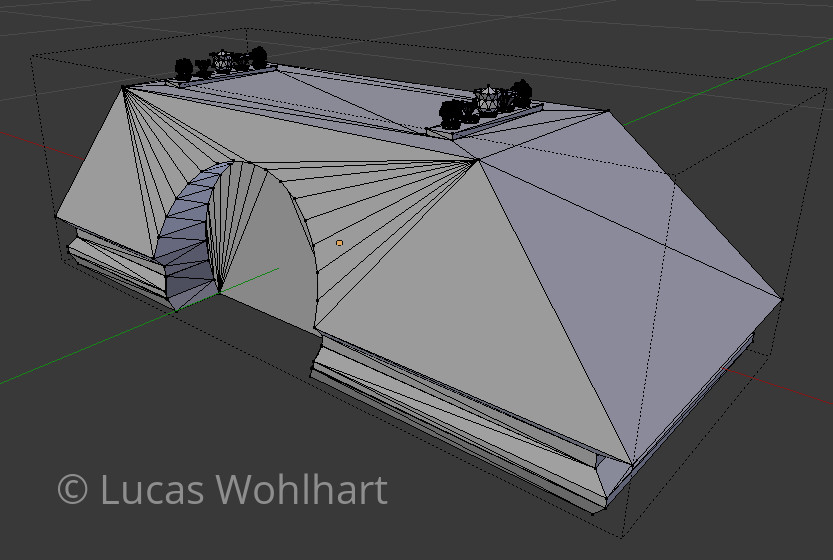
\includegraphics[width=\linewidth]{img/blender_mse6_chassis}
      \caption{Blender: MSE6 chassis design}
      \label{fig:blender_design_mse6}
\end{figure}

\begin{table}[h]
      \caption{lw\_mse6\_bot model}
      \label{tab:lw_mse6_bot_model}
      \begin{center}
            \begin{tabular}{|l||c|c|} 
                  \hline
                  Part & Geometry & Dimension\\ \hline \hline
                  Chassis & Mesh &  \\ 
                        & Outer-Dimensions & 0.675 x 0.3 x 0.236 \\
                        & Origin & x: 0.0375 y: 0.0 z: 0.062 \\ \hline 
                  Back/Front caster & Sphere & radius: 0.0499 \\ 
                  & Origin & x: $\pm$ 0.15 y: 0.0 z: -0.05 \\ \hline 
                  Left/Right Wheel & Cylinder & radius: 0.1, height: 0.05 \\ 
                  & Origin & x: 0.0 y: $\pm$ 0.15 z: 0.0 \\ \hline \hline  
                  Camera Sensor & Cube &  0.05 x 0.05 x 0.05\\ 
                  & Origin & x: 0.3 y: 0.0 z: 0.08 \\ \hline 
                  Laser Range Sensor & Mesh &  0.1 x 0.1 x 0.1\\ 
                  (Hokuyo)  & Origin & x: 0.2 y: 0.0 z: 0.15 \\ \hline  
            \end{tabular}
      \end{center}
\end{table}

The chassis is placed on a a back- and front-caster for stability and linked to two cylindrical wheels resulting in a differential drive robot. The laser range sensor is mounted on top of the chassis and the camera sensor sits on front of the robot.
The entire robot is depicted in Figure~\ref{fig:mse6_bot} and the dimensions are declared in Table~\ref{tab:lw_mse6_bot_model}.


\begin{figure}[thpb]
      \centering
      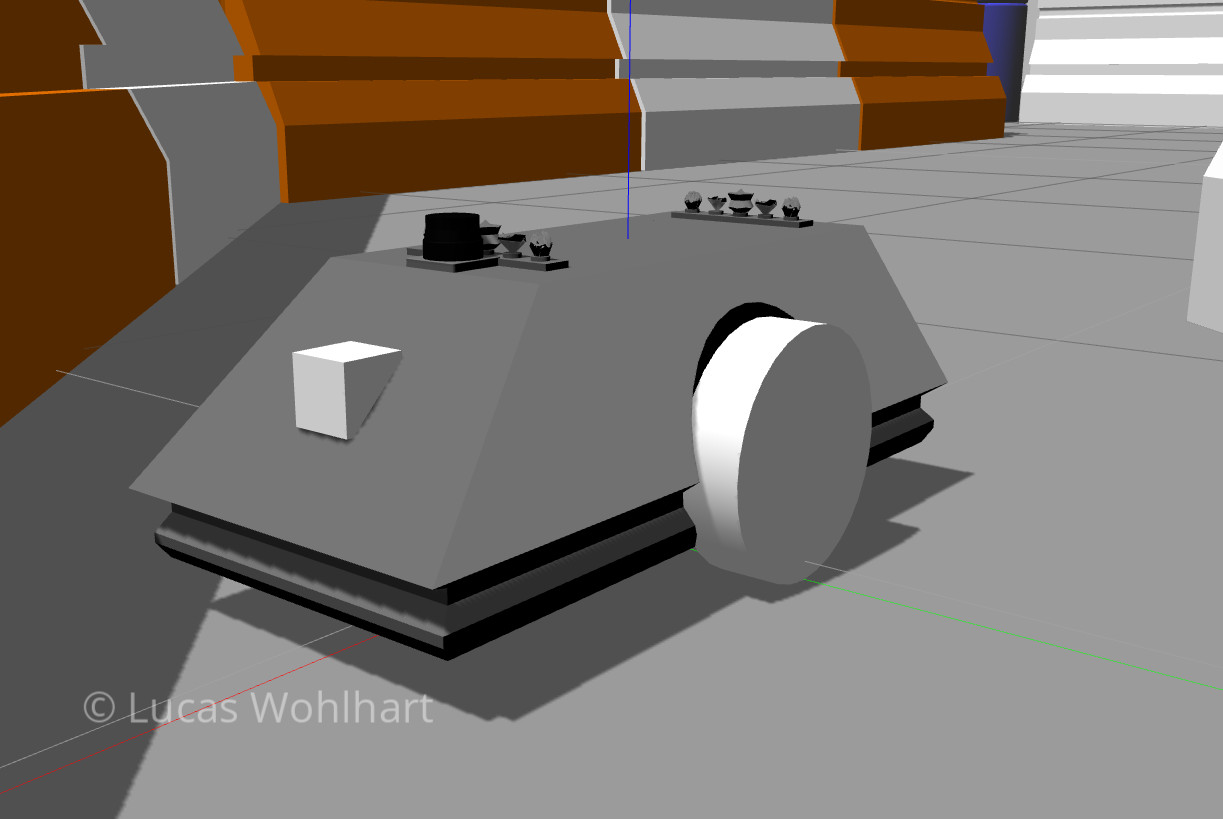
\includegraphics[width=\linewidth]{img/lw_mse6_bot}
      \caption{MSE6 Bot}
      \label{fig:mse6_bot}
\end{figure}
\subsubsection{Packages Used}
The MSE6 bot uses the same ROS packages as the udacity\_bot described in section~\ref{sec:packages_udacity_bot}

\subsubsection{Parameters}
Most of the parameterization used for the udacity\_bot works for the MSE6 bot, but the newly introduced geometry of the chassis requires adaptation of the costmap common parameters.
Since the robots hitbox can't be approximated by a circle anymore it's necessary to declare its \texttt{footprint} instead of the \texttt{robot\_radius}.
Additionally it has proven to be beneficial to increase the \texttt{inflation\_radius} to 0.7 to prevent obstacle collisions.
\begin{table}[h]
      \begin{center}
            \begin{tabular}{|l|c|c|} 
      \multicolumn{2}{c}{costmap common parameters} \\ \hline
      footprint & [[0.375, 0.25], [0.375, -0.25], [-0.3, -0.25], [-0.3, 0.25]] \\ \hline
      inflation\_radius & 0.7 \\ \hline
\end{tabular}
\end{center}
\end{table}


In order to stop the hokuyo laser range sensor from hitting parts of the chassis the minimum range of gazebo configuration for the hokuyo sensor had to be increased to 0.15.

\section{Results}

Present an unbiased view of your robot's performance and justify your stance with facts. Do the localization results look reasonable? What is the duration for the particle filters to converge? How long does it take for the robot to reach the goal? Does it follow a smooth path to the goal? Does it have unexpected behavior in the process? \\
For demonstrating your results, it is incredibly useful to have some watermarked charts, tables, and/or graphs for the reader to review. This makes ingesting the information quicker and easier.

\subsection{Localization Results}
\subsubsection{Benchmark}
\begin{figure}[thpb]
      \centering
      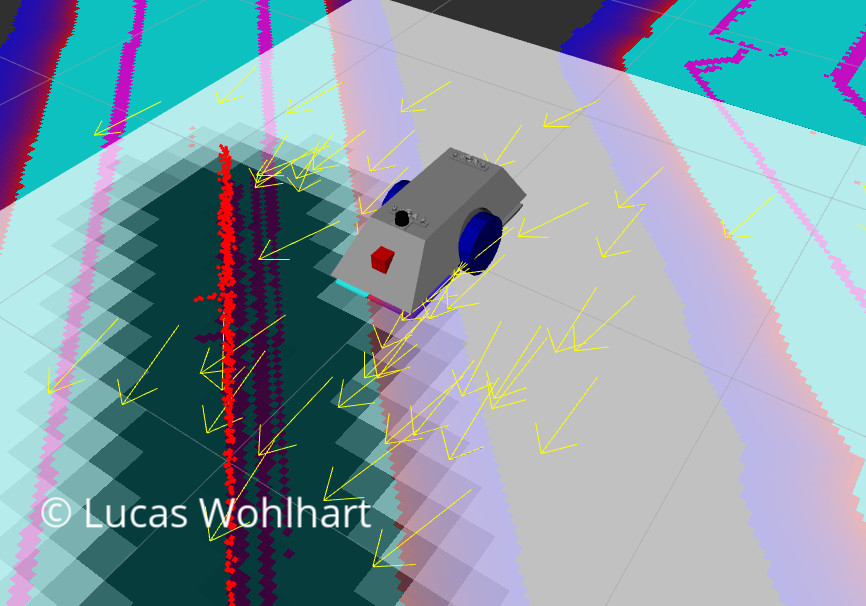
\includegraphics[width=\linewidth]{img/particles_initial}
      \caption{Initial AMCL particles}
      \label{fig:initial_amcl_particles}
\end{figure}
\begin{figure}[thpb]
      \centering
      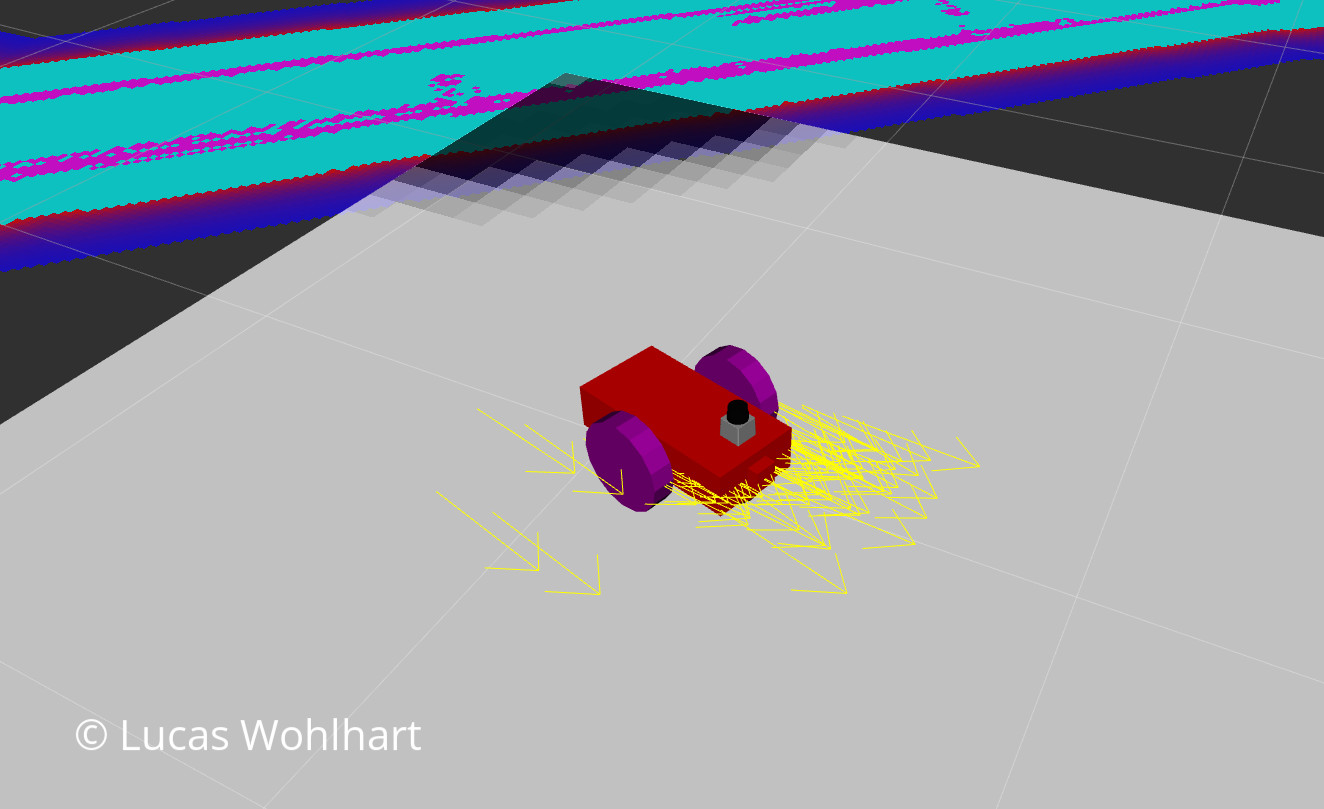
\includegraphics[width=\linewidth]{img/udacity_bot_goal_location}
      \caption{Udacity Bot at goal location}
      \label{fig:udacity_bot_goal_location}
\end{figure}




\subsubsection{Student}

\begin{figure}[thpb]
      \centering
      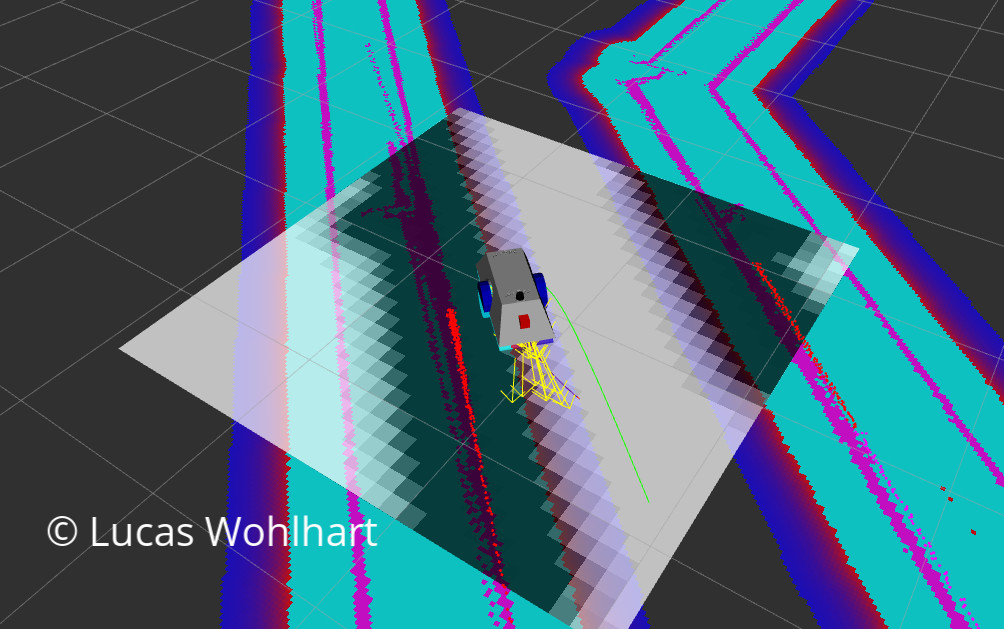
\includegraphics[width=\linewidth]{img/lw_mse6_bot_particles_converged}
      \caption{AMCL particles converging}
      \label{fig:amcl_particles_converging}
\end{figure}
\begin{figure}[thpb]
      \centering
      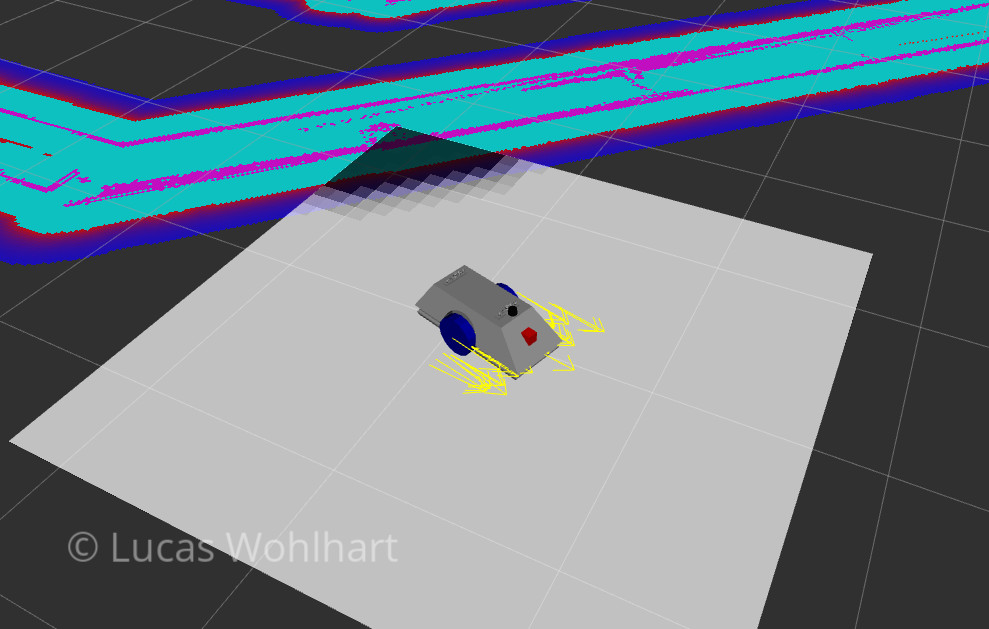
\includegraphics[width=\linewidth]{img/lw_mse6_bot_goal_location}
      \caption{MSE6 Bot at goal location}
      \label{fig:mse6_bot_goal_location}
\end{figure}

\subsection{Technical Comparison} % only facts
Discuss the difference of the layout, parameters, performance etc. between the benchmark robot and your robot. It is acceptable for your custom robot to perform worse than the provided robot. The focus is on learning and understanding, not performance. 

\section{Discussion}
This is the only section of the report where you may include your opinion. However, make sure your opinion is based on facts. If your robot performed poorly, make mention of what may be the underlying issues. If the robot runs well, which aspects contribute to that? Again, avoid writing in the first person (i.e. Do not use words like "I" or "me"). If you really find yourself struggling to avoid the word "I" or "me"; sometimes, this can be avoid with the use of the word “one”. As an example: instead of : "I think the robot cannot localize itself because the sensor does not provide enough information for localization" try: "one may believe the localization performance is poor because the sensor layout is not able to provide enough information for localization". They say the same thing, but the second avoids the first person. 

\subsection{Topics}
\begin{itemize}
\item Which robot performed better?
\item Why it performed better? (opinion)
\item How would you approach the 'Kidnapped Robot' problem?
\item What types of scenario could localization be performed?
\item Where would you use MCL/AMCL in an industry domain?
\end {itemize}

\section{Conclusion / Future work}
This section is intended to summarize your report. Your summary should include a recap of the results, did this project achieve what you attempted, how would you deploy it on hardware and how could this project be applied to commercial products? 
For Future Work, address areas of work that you may not have addressed in your report as possible next steps. This could be due to time constraints, lack of currently developed methods / technology, and areas of application outside of your current implementation. Again, avoid the use of the first-person.

\subsection{Modifications for Improvement}
Examples:
\begin{itemize}
\item Base Dimension
\item Sensor Location
\item Sensor Layout
\item Sensor Amount
\end{itemize}


\bibliography{bib}
\bibliographystyle{ieeetr}

\end{document}